\documentclass[a4paper]{article}

\usepackage{INTERSPEECH2016}

\usepackage{graphicx}
\usepackage{amssymb,amsmath,bm}
\usepackage{textcomp}
 \usepackage{hyperref}
 \usepackage{multirow}
\usepackage{array}

\def\vec#1{\ensuremath{\bm{{#1}}}}
\def\mat#1{\vec{#1}}


\sloppy % better line breaks
\ninept

\title{An Improved Residual LSTM Architecture for Acoustic Modeling}

%%%%%%%%%%%%%%%%%%%%%%%%%%%%%%%%%%%%%%%%%%%%%%%%%%%%%%%%%%%%%%%%%%%%%%%%%%
%% If multiple authors, uncomment and edit the lines shown below.       %%
%% Note that each line must be emphasized {\em } by itself.             %%
%% (by Stephen Martucci, author of spconf.sty).                         %%
%%%%%%%%%%%%%%%%%%%%%%%%%%%%%%%%%%%%%%%%%%%%%%%%%%%%%%%%%%%%%%%%%%%%%%%%%%
%\makeatletter
%\def\name#1{\gdef\@name{#1\\}}
%\makeatother
%\name{{\em Firstname1 Lastname1, Firstname2 Lastname2, Firstname3 Lastname3,}\\
%      {\em Firstname4 Lastname4, Firstname5 Lastname5, Firstname6 Lastname6,
%      Firstname7 Lastname7}}
%%%%%%%%%%%%%%% End of required multiple authors changes %%%%%%%%%%%%%%%%%

\makeatletter
\def\name#1{\gdef\@name{#1\\}}
\makeatother \name{{\em Lu Huang$^1$, Jiasong Sun$^1$, Ji Xu$^2$, Yi Yang$^1$}}

\address{$^1$Department of Electronic Engineering, Tsinghua University, Beijing, China \\
  $^2$Key Laboratory of Speech Acoustics and Content Understanding, \\Chinese Academy of Sciences, Beijing, China \\
  {\small \tt huanglu.th@gmail.com, xuji@hccl.ioa.ac.cn, \{sunjiasong,yangyy\}@tsinghua.edu.cn}
}

%\twoauthors{Karen Sp\"{a}rck Jones.}{Department of Speech and Hearing \\
%  Brittania University, Ambridge, Voiceland \\
%  {\small \tt Karen@sh.brittania.edu} }
%  {Rose Tyler}{Department of Linguistics \\
%  University of Speechcity, Speechland \\
%  {\small \tt RTyler@ling.speech.edu} }

%
\begin{document}

  \maketitle
  %
  \begin{abstract}
Long Short-Term Memory (LSTM) is the primary recurrent neural networks architecture for acoustic modeling in automatic speech recognition systems.
Residual learning is an efficient method to help neural networks converge easier and faster.
In this paper, we propose several types of residual LSTM  methods for our acoustic modeling.
Our experiments indicate that, compared with classic LSTM, our architecture has more than 8\% relative reduction in Word Error Rate (WER) on TIMIT tasks.
At the same time, our residual fast LSTM approach shows 4\% relative reduction in WER on the same task.
Besides, we find that all these methods could have good results on THCHS-30 corpus.
  \end{abstract}
  \noindent{\bf Index Terms}: long short-term memory, residual learning, acoustic modeling, speech recognition



  \section{Introduction}

GRU 
\begin{equation}
z_t = \sigma ( U_z*x_t + W_z*s_{t-1} ) 
\end{equation}
\begin{equation}
r_t = \sigma (U_r* x_t   + W_r*s_{t-1}  )
\end{equation}
\begin{equation}
h_t = \tanh ( U_h*x_t  + W_h*(s_{t-1} \odot r_t) )
\end{equation}
\begin{equation}
s_t = ( 1 - z_t ) \odot h_t + z_t \odot s_{t-1}
\end{equation}
\begin{equation}
y_t=W_{p}*s_t
\end{equation}
\begin{equation}
s_t={y_t}(1:n_r)
\end{equation}



Artificial Neural Networks (ANNs) had been widely researched in many Automatic Speech Recognition (ASR) systems for a long time.
Since the year of 2011, Microsoft proposed its first deep neural networks which extremely improved the performance of speech recognition system \cite{ms-dnn}.
After that, Deep Neural Networks (DNNs), Convolution Neural Networks (CNNs) and Recurrent Neural Networks (RNNs) have been the most important research and development ways and tools.
But there are still some problems on training deeper network for the existence of vanishing gradients and exploding gradients \cite{gradient}.
The standard LSTM-RNNs \cite{lstm} has been designed to address these problems \cite{lstm-asr}.


At the same time, the residual networks have been applied in image recognition \cite{res-image} and speech recognition \cite{residual-lstm,IBM-5.5,MS-1,MS-2,res-lstm}.
Especially, residual LSTM is proposed to improve the performance of speech recognition systems \cite{residual-lstm,res-lstm}.
Meanwhile, fast LSTM \cite{fast-lstm-1,fast-lstm-2} is proposed to reduce the training time without sacrificing performance, sometimes even with improved performance.


In this paper, inspired by Residual LSTM in \cite{residual-lstm},
we propose an improved residual LSTM to replace vector's addition by splicing vector with various shortcut connection locations.
They have good performance  as the acoustic modeling on TIMIT \cite{timit} and THCHS-30 \cite{thchs30} tasks.


We start by describing some fundamental LSTM architectures in Section 2,
including standard LSTM, projected LSTM \cite{lstm-asr}, fast LSTM and residual LSTM \cite{residual-lstm}.
Then the improved residual LSTM is proposed in Section 3.
After that, we provide some experiments and results on TIMIT and THCHS-30 corpora in Section 4, which is followed by conclusions in Section 5.


  \section{Fundamental LSTM-related Architectures}
\label{sec:lstm}
Since LSTM was proposed in \cite{lstm}, it has achieved significant performance in sequence labelling and prediction \cite{seq-lab},
especially as acoustic modeling and language modeling in ASR systems.

In this section, some LSTM-related works are provided, included projected LSTM, fast LSTM, and residual LSTM \cite{residual-lstm}.

\subsection{LSTM}

In the year of 2014, the projected LSTM is proposed by Google for speech recognition \cite{lstm-asr},
which is called LSTM projected (LSTMP) architecture in some other literatures.
When compared with the standard LSTM, projected LSTM add a projection layer to the output,
and also the recurrent vector is truncated from the output vector in Kaldi \cite{kaldi}, as illustrated in Fig.1 and shown by the following equations.
\begin{figure}
\centering
  \includegraphics[width=3.0in]{lstmp-kaldi.eps}
  \caption{The projected LSTM in Kaldi.}
\end{figure}
\begin{equation}\label{1}
i_t=\sigma(W_{ix}x_t+W_{ir}r_{t-1}+W_{ic}c_{t-1}+b_i)
\end{equation}
\begin{equation}\label{2}
f_t=\sigma(W_{fx}x_t+W_{fr}r_{t-1}+W_{fc}c_{t-1}+b_f)
\end{equation}
\begin{equation}\label{3}
g_t=\tanh(W_{cx}x_t+W_{cr}r_{t-1}+b_c)
\end{equation}
\begin{equation}\label{4}
c_t=f_t\odot c_{t-1}+i_t\odot g_t
\end{equation}
\begin{equation}\label{5}
o_t=\sigma(W_{ox}x_t+W_{or}r_{t-1}+W_{oc}c_{t}+b_o)
\end{equation}
\begin{equation}\label{6}
m_t=o_t\odot \tanh(c_t)
\end{equation}
\begin{equation}\label{7}
y_t=W_{rp}m_t
\end{equation}
\begin{equation}\label{8}
r_t={y_t}(1:n_r)
\end{equation}
Where the $W$ represents weight matrix and the $b$ is bias vector. For example, $W_{ic}$ is the matrix of weights from cell activation vectors to input gate,
$b_i$ is the bias vector of input gate. $i_t$, $f_t$ and $o_t$ are the input gate, forget gate and output gate respectively.
$c_t$ and $m_t$ are cell activation vector and cell output activation vector.
All of $i_t$, $f_t$, $o_t$, $c_t$ and $m_t$ are the same size. Besides, $g_t$ is the processed input, $r_t$ is for recurrence, $y_t$ is the output, $W_{rp}$ is the projection matrix.
$\odot$ stands for element-wise multiplication, ${y_t}(1:n_r)$ means that $r_t$ is the first $n_r$ elements of $y_t$.

%The projected LSTM mentioned above is widely used in speech recognition, which is selected as our baseline to compare with.

\subsection{Fast LSTM}

LSTM-RNN has more complexity than general RNN, which leads to a slower training speed.
To accelerate its training, several algorithms have been done in previous work \cite{fast-lstm-1,fast-lstm-2,miao-lstm},
in which the fast LSTM \cite{fast-lstm-1,fast-lstm-2} can cut down half training time with incidentally improvement of performance.
Compared to LSTM, fast LSTM doesn't use $c_t$ or $c_{t-1}$ to compute $i_t$, $f_t$ and $o_t$, as shown in the following equations.
\begin{equation}\label{9}
i_t=\sigma(W_{ix}x_t+W_{ir}r_{t-1}+b_i)
\end{equation}
\begin{equation}\label{10}
f_t=\sigma(W_{fx}x_t+W_{fr}r_{t-1}+b_f)
\end{equation}
\begin{equation}\label{11}
o_t=\sigma(W_{ox}x_t+W_{or}r_{t-1}+b_o)
\end{equation}

Obviously, equation (9), (10), (11) and (3) have the same inner operation, except that the active function is different for equation (3).
Since these four equations have the same inner operation and inputs, a larger matrix is adopted in Kaldi to convert them into one operation with a large output,
which contains four parts to represent the inputs of active functions: $i_t$, $f_t$, $o_t$ and $g_t$.
This kind of large matrix is more suitable for Graphics Processing Unit (GPU) computing than small matrices when they have the same amount of parameters.

\subsection{Residual LSTM}

As mentioned above, the DNN's training will become harder with the increase of depth.
The reason is attributed to vanishing gradients and exploding gradients.
Residual learning has been proposed to solve these problems in image recognition \cite{res-image}, and recently in speech recognition \cite{residual-lstm,res-lstm}.

The output of each layer is the sum of network's input and network's output in \cite{res-lstm}, i.e., there is one shortcut connection between network's input and output,
which has the same form as on most image recognition tasks.
However, the shortcut connection is ended at one network's interior node, instead of network's output in \cite{residual-lstm}.



\section{The Improved Residual LSTM Architectures}

Inspired by the principle in \cite{residual-lstm}, our LSTM architectures have a short connection in LSTM on three different locations.
Two of them are inner nodes and one of them is output, which is shown in Fig.2. Besides, we replace vector's addition by splicing vector in each location,
and then project the spliced vector to the original dimension in location 1 and 3 to prevent the exploding dimension of vectors.
In location 2, we reuse the projection matrix $W_{rp}$ by increasing its input dimension.
\begin{figure}
\centering
  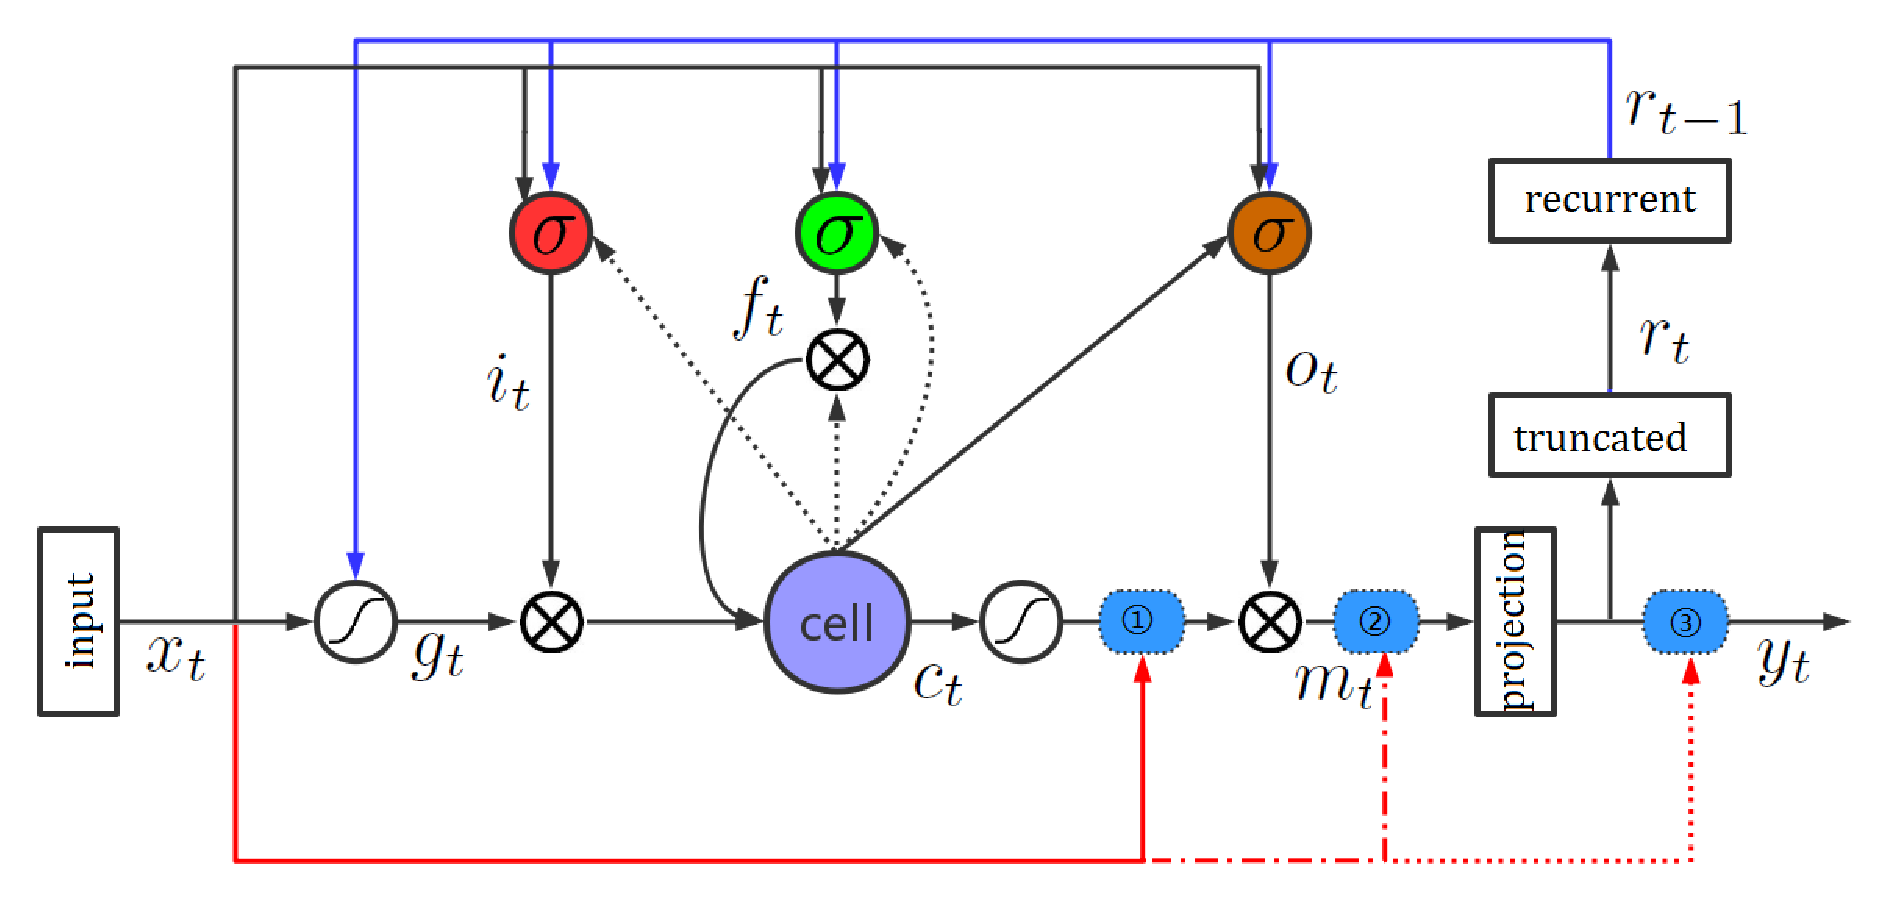
\includegraphics[width=3.0in]{lstmp.eps}
  \caption{The improved residual LSTM with a shortcut connection from input to the later node and there are three locations.
   }
\end{figure}

When the junction is located at position 1, as shown in Fig.2, we name our improved Residual LSTM as LSTM Res-1, and the same is true for LSTM Res-2 and LSTM Res-3.
So compared to the original LSTM, our first method LSTM Res-1 has different equations from equation (6) as below.
\begin{equation}\label{12}
h_t=(\tanh(c_t), x_t)
\end{equation}
\begin{equation}\label{13}
m_t=o_t\odot (W_{res1}h_t)
\end{equation}
Where $h_t$ is the spliced vector, $W_{res1}$ is the projection matrix. Our second method LSTM Res-2 has different equations from equation (7) as below.
\begin{equation}\label{14}
h_t=(m_t, x_t)
\end{equation}
\begin{equation}\label{15}
y_t=W_{res2}h_t
\end{equation}
Where $W_{res2}$ is the projection matrix for replacing $W_{rp}$ in equation (7). Similarly, the third one LSTM Res-3 changes equation (7) and (8) into following equations.
\begin{equation}\label{16}
z_t=W_{rp}m_t
\end{equation}
\begin{equation}\label{17}
r_t=z_t(1:n_r)
\end{equation}
\begin{equation}\label{18}
h_t=(z_t, x_t)
\end{equation}
\begin{equation}\label{19}
y_t=W_{res3}h_t
\end{equation}
Where $z_t$ is an intermediate vector, $W_{res3}$ is the projection matrix.


Since fast LSTM is faster to train, we also examine these thoughts into fast LSTM and test their performance on TIMIT and THCHS-30 tasks.

\section{Experiments}

We use nnet3 recipes in Kaldi, a popular toolkit for speech recognition, to implement our LSTM architectures.
The input of neural networks is a 300 dimensional vector,
consisting of 40 dimensional MFCC (Mel Frequency Cepstral Coefficient) features without cepstral truncation of five frames,
which are spliced across in $\pm 2$ frames of context, and 100 dimensional i-vectors to perform speaker adaptation \cite{ivector}.

Here all the implemented LSTM architectures have 2, 3 or 4 LSTM layers followed by a fully connected layer and a softmax layer.
They are trained by cross-entropy (CE) criterion \cite{ce}.
We use dual Nvidia GPUs to accelerate the training based on the parallel algorithm proposed in \cite{kaldi-gpus}.

In order to evaluate our recipes quickly, speed perturbation \cite{audio-aug} is not considered in our system.
Speed perturbation is adopted to generate more training data for audio augmentation in Kaldi by default,
but its performance improvement is very limited.

Since the training of LSTM is very slow, LSTM is just operated on TIMIT task.
And these thoughts with fast LSTM are evaluated on THCHS-30 task.


\subsection{On TIMIT Task}

TIMIT Speech Corpus \footnote{There are more details on website: \url{https://catalog.ldc.upenn.edu/ldc93s1}.} is widely used in acoustic-phonetic studies.
in our experiments, 3.14 hours of data was selected as training data, with 0.16 hours as core test set and 0.81 hours as a complete test set,
which was suggested by official \cite{timit-off}. The core test set is the subset of the complete test set.

The baseline LSTM implemented on TIMIT is the projected LSTM provided by Kaldi and Residual LSTM \cite{residual-lstm}.
All LSTM, fast LSTM and their residual architectures have 1024-dimensional cell,
with 512-dimensional recurrent projection and zero-dimensional no-recurrent projection,
i.e., all elements of $y_t$ is used for recurrence.
Residual LSTM is the architecture proposed in \cite{residual-lstm}.
All neural networks are trained for 15 epochs for the amount of training data is very small.
The results are illustrated in Table 1\footnote{The depth here is the number of LSTM layers. \#D means depth of LSTM, and \#P stands for the amount of parameters.}.

\begin{table}
\caption{Results of TIMIT Task (WER\%)}
\centering
\begin{tabular}{c|c|c|c|c}
%\begin{tabular}{m{2.7cm}<{\centering}|m{1.3cm}<{\centering}|m{2.5cm}<{\centering}|m{2cm}<{\centering}|m{2.5cm}<{\centering}}
\hline%\hline
\textbf{AM Types} & \textbf{\#D} & \textbf{\#P} & \textbf{core} & \textbf{complete} \\ \hline\hline
\multirow{3}{2.4cm}{\centering{LSTM}} & 2 & 9.6M& 21.0&20.3 \\ %\cline{2-5}
& 3 & 14.3M&21.2 &\textbf{20.0} \\ %\cline{2-5}
& 4 & 19.0M&\textbf{20.8} &20.1 \\ \hline
\multirow{3}{2.4cm}{\centering{Residual LSTM \cite{residual-lstm}}} & 2 &9.8M &21.4 &20.4 \\
& 3 &14.6M &20.8 &20.1 \\ %\cline{2-5}
& 4 &19.3M &\textbf{20.7} &\textbf{19.7} \\ \hline
\multirow{3}{2.4cm}{\centering{LSTM Res-1}} & 2 &12.5M &20.0 &19.1 \\ %\cline{2-5}
& 3 & 18.8M& 20.0&18.7 \\ %\cline{2-5}
& 4 & 25.1M& \textbf{19.3}&\textbf{18.4} \\ \hline
\multirow{3}{2.4cm}{\centering{LSTM Res-2}} & 2 &10.0M &21.2 &19.8 \\ %\cline{2-5}
& 3 &15.0M &\textbf{19.8} &19.3 \\ %\cline{2-5}
& 4 &20.0M &20.2 &\textbf{19.1} \\ \hline
\multirow{3}{2.4cm}{\centering{LSTM Res-3}} & 2 &10.5M &20.1 &19.1 \\ %\cline{2-5}
& 3 &15.8M &\textbf{19.9} &18.8 \\ %\cline{2-5}
& 4 &21.0M &20.2 &\textbf{18.6} \\ \hline
\multirow{3}{2.4cm}{\centering{Fast LSTM}} & 2 &9.6M &20.3 &19.3 \\ %\cline{2-5}
& 3 &14.3M &20.1 &18.7 \\ %\cline{2-5}
& 4 &19.0M &\textbf{20.0} &\textbf{18.7} \\ \hline
\multirow{3}{2.4cm}{\centering{Fast LSTM Res-1}} & 2 & 12.5M&19.5 &18.5 \\ %\cline{2-5}
& 3 &18.8M &\textbf{19.2} &\textbf{18.1} \\ %\cline{2-5}
& 4 &25.1M &19.5 &\textbf{18.1} \\ \hline
\multirow{3}{2.4cm}{\centering{Fast LSTM Res-2}} & 2 &10.0M &19.9 &18.6 \\ %\cline{2-5}
& 3 &15.0M &\textbf{19.3} &18.2 \\ %\cline{2-5}
& 4 &20.0M &19.6 &\textbf{17.9} \\ \hline
\multirow{3}{2.4cm}{\centering{Fast LSTM Res-3}} & 2 &10.5M &19.6 &18.7 \\ %\cline{2-5}
& 3 &15.8M &\textbf{19.2} &18.2 \\ %\cline{2-5}
& 4 &21.0M &19.3 &\textbf{18.0} \\ \hline
\end{tabular}
\end{table}

According to the matrix $W_{ic}$, $W_{fc}$ and $W_{oc}$ in equation (1), (2) and (5), which are all diagonal matrices
and have very small amount of parameters when compared them with other general matrices such as $W_{ix}$ and $W_{ir}$,
the number of parameters of LSTM is approximately equal to fast LSTM.

As shown in Table 1, Residual LSTM proposed in \cite{residual-lstm} has a very small improvement in performance;
the residual methods we proposed outperform both baseline LSTM and Residual LSTM,
with a relative reduction in WER about 8\% on complete test set for LSTM Res-1.
Besides, fast LSTM is not only faster than standard LSTM, but also outperform  standard LSTM.

When applied to fast LSTM, our residual recipes also gain performance improvement,
with a relative reduction in WER about 4\% on both core test set and complete test set.
More importantly, our fast LSTM Res recipes have the best performance.
So on the following THCHS-30 task, we just apply these three ideas to fast LSTM.

\subsection{On THCHS-30 Task}

THCHS-30 (Tsinghua Chinese 30-hour database) is a free and open-source Chinese speech database\footnote{There are more details on website:
\url{http://data.cslt.org/thchs30/README.html}.}.
On this task, we use about 27 hours of data for training and about 6 hours of data for testing \cite{thchs30}.


Different with TIMIT task, the baseline fast LSTM and the three residual fast LSTM recipes here are implemented with 1024-dimensional cell,
256-dimensional recurrent projection and 256-dimensional no-recurrent projection.
Besides, we train all neural networks for 8 epochs.
When decoding, we perform both phone decoding and word decoding, which convert the speech signal into phone sequences and word sequences.
The results are shown in Table 2\footnote{PER means phone error rate. WER is for word decoding, and PER is for phonetic decoding.}.

\begin{table}
\caption{Results of THCHS-30 Task (WER\%/PER\%)}
\centering
\begin{tabular}{c|c|c|c|c}
%\begin{tabular}{m{2.7cm}<{\centering}|m{1.3cm}<{\centering}|m{2.4cm}<{\centering}|m{2.4cm}<{\centering}|m{2.4cm}<{\centering}}
\hline
\textbf{AM Types} & \textbf{\#D} & \textbf{\#P} & \textbf{word} & \textbf{phone} \\ \hline \hline
\multirow{3}{2.4cm}{\centering Fast LSTM     } &2 & 8.2M &22.94 &9.53 \\
  &3 &11.9M &22.74 &9.15 \\
  &4 &15.6M &\textbf{22.62} &\textbf{9.01} \\ \hline
\multirow{3}{2.4cm}{\centering Fast LSTM Res-1} &2 &11.2M &23.29 &9.13 \\
  &3 &16.4M &22.97 &8.87 \\
  &4 &21.7M &\textbf{22.83} &\textbf{8.74} \\ \hline
\multirow{3}{2.4cm}{\centering Fast LSTM Res-2} &2 & 8.6M &22.64 &9.31 \\
  &3 &12.6M &22.36 &8.75 \\
  &4 &16.5M &\textbf{22.15} &\textbf{8.38} \\ \hline
\multirow{3}{2.4cm}{\centering Fast LSTM Res-3} &2 & 9.2M &22.92 &8.88 \\
  &3 &13.4M &22.57 &8.72\\
  &4 &17.6M &\textbf{22.40} &\textbf{8.31} \\ \hline
\end{tabular}
\end{table}

Obviously, the recipes we proposed outperform the standard fast LSTM in most cases, especially on phone task.
And in several cases, there are about 7\% relative improvement of performance on phone task and about 2\% relative improvement of performance on word task.

Meanwhile, the best result provided by CSLT@THU is 23.18\% on word task and 10.01\% on phone task \cite{thchs-ch}.
And our best result is 22.15\% on word task and 8.31\% on phone task, with 4.4\% relative reduction in WER and 16.9\% relative reduction in PER.


\section{Conclusions}
In this paper, we propose our improved residual LSTM architectures for acoustic modeling.
The experiments on TIMIT corpus show that our recipes outperform the standard LSTM and the Residual LSTM proposed in \cite{residual-lstm},
with about 8\% reduction in WER on complete test set.
Also, we apply our thoughts to fast LSTM and achieve our best performance in both TIMIT corpus and THCHS-30 corpus.
Besides, the best performance was shown by using our fast LSTM structure on THCHS-30 task.

Next, we are interested in bidirectional LSTM \cite{blstm} and deeper LSTM.
We would also like improving performance on other corpora by using our improved residual LSTM architectures.

\section{Acknowledgments}
This work is partially supported by the National Natural Science Foundation of China (Nos. 11590770-4).

%  \newpage
  \eightpt
  \bibliographystyle{IEEEtran}

  \bibliography{mybib}

%  \begin{thebibliography}{99}
%    \bibitem{ms-dnn}
%Seide F, Li G, Yu D. Conversational Speech Transcription Using Context-Dependent Deep Neural Networks[C]. INTERSPEECH. 2011: 437-440.
%\bibitem {gradient}
%Bengio Y, Simard P, Frasconi P. Learning long-term dependencies with gradient descent is difficult[J]. IEEE transactions on neural networks, 1994, 5(2): 157-166.
%\bibitem{lstm}
%Hochreiter S, Schmidhuber J. Long short-term memory[J]. Neural computation, 1997, 9(8): 1735-1780.
%\bibitem{lstm-asr}
%Sak H, Senior A, Beaufays F. Long short-term memory based recurrent neural network architectures for large vocabulary speech recognition[J]. arXiv preprint arXiv:1402.1128, 2014.
%\bibitem {res-image}
%He K, Zhang X, Ren S, et al. Deep residual learning for image recognition[C]. Proceedings of the IEEE Conference on Computer Vision and Pattern Recognition. 2016: 770-778.
%\bibitem{residual-lstm}
%Kim J, El-Khamy M, Lee J. Residual LSTM: Design of a Deep Recurrent Architecture for Distant Speech Recognition[J]. arXiv preprint arXiv:1701.03360, 2017.
%\bibitem {IBM-5.5}
%Saon G, Kurata G, Sercu T, et al. English conversational telephone speech recognition by humans and machines[J]. arXiv preprint arXiv:1703.02136, 2017.
%\bibitem{MS-1}
%Xiong W, Droppo J, Huang X, et al. Achieving human parity in conversational speech recognition[J]. arXiv preprint arXiv:1610.05256, 2016.
%\bibitem{MS-2}
%Xiong W, Droppo J, Huang X, et al. The Microsoft 2016 conversational speech recognition system[J]. arXiv preprint arXiv:1609.03528, 2016.
%\bibitem{res-lstm}
%Zhang Y, Chan W, Jaitly N. Very deep convolutional networks for end-to-end speech recognition[J]. arXiv preprint arXiv:1610.03022, 2016.
%\bibitem{fast-lstm-1}
%Selvaraj S P P, Konam S. Deep Learning for Speaker Recognition[J].
%\bibitem{fast-lstm-2}
%Ogunmolu O, Gu X, Jiang S, et al. Nonlinear Systems Identification Using Deep Dynamic Neural Networks[J]. arXiv preprint arXiv:1610.01439, 2016.
%\bibitem{timit}
%Garofolo J S, Lamel L F, Fisher W M, et al. TIMIT Acoustic-Phonetic Continuous Speech Corpus LDC93S1. Philadelphia: Linguistic Data Consortium, 1993.
%\bibitem{thchs30}
%Wang D, Zhang X. THCHS-30: A free Chinese speech corpus[J]. arXiv preprint arXiv:1512.01882, 2015.
%\bibitem{swbd}
%Godfrey J J, Holliman E C, McDaniel J. SWITCHBOARD: Telephone speech corpus for research and development[C]. 1992 IEEE International Conference on Acoustics, Speech and Signal Processing. IEEE, 1992, 1: 517-520.
%\bibitem{seq-lab}
%Alex G. Supervised Sequence Labelling with Recurrent Neural Networks[D]. Munich: Technical University of Munich, 2008.
%\bibitem{kaldi}
%Povey D, Ghoshal A, Boulianne G, et al. The Kaldi speech recognition toolkit[C]. 2011 IEEE Workshop on Automatic Speech Recognition and Understanding. IEEE, 2011.
%\bibitem{miao-lstm}
%Miao Y, Li J, Wang Y, et al. Simplifying long short-term memory acoustic models for fast training and decoding[C]. 2016 IEEE International Conference on Acoustics, Speech and Signal Processing. IEEE, 2016: 2284-2288.
%\bibitem{ivector}
%Saon G, Soltau H, Nahamoo D, et al. Speaker adaptation of neural network acoustic models using i-vectors[C]. 2013 IEEE Workshop on Automatic Speech Recognition and Understanding. IEEE, 2013: 55-59.
%\bibitem{ce}
%De Boer P T, Kroese D P, Mannor S, et al. A tutorial on the cross-entropy method[J]. Annals of operations research, 2005, 134(1): 19-67.
%\bibitem{kaldi-gpus}
%Povey D, Zhang X, Khudanpur S. Parallel training of deep neural networks with natural gradient and parameter averaging[J]. arXiv preprint, 2014.
%\bibitem{audio-aug}
%Ko T, Peddinti V, Povey D, et al. Audio augmentation for speech recognition[C]. INTERSPEECH. 2015: 3586-3589.
%\bibitem{timit-off}
%Lopes C, Perdigao F. Phone recognition on the TIMIT database[J]. Speech Technologies/Book, 2011, 1: 285-302.
%\bibitem{thchs-ch}
%THCHS-30 CHALLENGE, (Accessed April 19, 2017). [Online]. Available: \url{http://data.cslt.org/thchs30/challenges/asr.html}.
%\bibitem{blstm}
%Graves A, Jaitly N, Mohamed A. Hybrid speech recognition with deep bidirectional LSTM[C]. 2013 IEEE Workshop on Automatic Speech Recognition and Understanding. IEEE, 2013: 273-278.

  %\end{thebibliography}

\end{document}
